% !TeX program = pdflatex
% !TeX encoding = UTF-8
% Manuscrito completo. As ilustrações são desenhadas em TikZ.
% Para compilar (incluindo os marcadores de navegação):
%   latexmk -pdf O_que_se_aprende_com_uma_cara.tex


\documentclass[11pt,oneside]{article}
\usepackage[T1]{fontenc}
\usepackage[utf8]{inputenc}
\usepackage[sc]{mathpazo}
\usepackage{amsmath,amssymb,booktabs,microtype}
\usepackage[paperwidth=165mm,paperheight=235mm,left=22mm,right=21mm,top=20mm,bottom=22mm,headheight=14pt,headsep=7mm,footskip=12mm]{geometry}
\usepackage{xcolor,tikz,fancyhdr,titlesec,needspace,environ}
\usepackage[unicode,hidelinks]{hyperref}
\hypersetup{pdfauthor={Caio Gomes},pdftitle={O que se aprende com uma cara},pdfsubject={Aprendizado de máquina, atualização de probabilidades e modelos de classificação. Capítulos 1 a 7.},pdflang={pt-BR},bookmarksopen=true,bookmarksnumbered=false,pdfdisplaydoctitle=true}
\definecolor{tinta}{HTML}{224D50}
\definecolor{leve}{HTML}{B9CFCC}
\definecolor{papel}{HTML}{F4F7F6}
\urlstyle{same}
\pagestyle{fancy}\fancyhf{}
\fancyhead[R]{\footnotesize\itshape\nouppercase{\rightmark}}\fancyfoot[C]{\small\thepage}
\renewcommand{\headrulewidth}{0pt}
\fancypagestyle{opening}{\fancyhf{}\fancyfoot[C]{\small\thepage}\renewcommand{\headrulewidth}{0pt}}
\setlength{\parindent}{1.22em}\setlength{\parskip}{0pt}\linespread{1.07}
\setlength{\emergencystretch}{1.7em}
\interfootnotelinepenalty=10000\clubpenalty=10000\widowpenalty=10000\displaywidowpenalty=10000
\titleformat{\subsection}{\large\bfseries}{}{0pt}{}
\titlespacing*{\subsection}{0pt}{13pt plus 3pt minus 3pt}{5.5pt}
\setcounter{secnumdepth}{0}\raggedbottom
\newcommand{\F}{\mathcal F}
\newcommand{\alinhamentodotitulo}{\raggedright}
\newcommand{\capitulo}[2]{\clearpage\thispagestyle{opening}\markright{#2}\pdfbookmark[0]{Capítulo #1 · #2}{ch#1}\noindent{\small\color{tinta}\textsc{Capítulo #1}\par}\vspace{6pt}{\alinhamentodotitulo\noindent\fontsize{24}{27}\selectfont\bfseries #2\par}\vspace{13pt}\noindent\ignorespaces}
\newcommand{\secao}[1]{\Needspace{5.2\baselineskip}\subsection*{#1}}
\newcommand{\itemq}[1]{\par\textbf{#1.}\enspace}
\NewEnviron{quadro}[1]{\par\addvspace{9pt}\begingroup\setlength{\fboxsep}{8pt}\setlength{\fboxrule}{.55pt}\noindent\fcolorbox{tinta}{papel}{\begin{minipage}{\dimexpr\linewidth-2\fboxsep-2\fboxrule\relax}\small\setlength{\parindent}{0pt}\setlength{\parskip}{3pt}{\large\bfseries\color{tinta}#1\par}\vspace{1pt}\BODY\end{minipage}}\par\endgroup\addvspace{9pt}}
\newcommand{\mesas}{%
\par\addvspace{7pt}\noindent\begin{minipage}{\linewidth}\centering
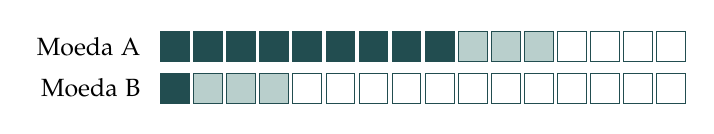
\begin{tikzpicture}[x=.42cm,y=.44cm,font=\small]
\node[anchor=east] at (-.32,1.49) {Moeda A};
\node[anchor=east] at (-.32,.29) {Moeda B};
\foreach \j in {0,...,15}{
 \ifnum\j<9 \def\filla{tinta}\else\ifnum\j<12 \def\filla{leve}\else\def\filla{white}\fi\fi
 \ifnum\j<1 \def\fillb{tinta}\else\ifnum\j<4 \def\fillb{leve}\else\def\fillb{white}\fi\fi
 \filldraw[fill=\filla,draw=tinta, line width=.35pt] (\j,1.04) rectangle +(0.87,.87);
 \filldraw[fill=\fillb,draw=tinta, line width=.35pt] (\j,-.16) rectangle +(0.87,.87);
}
\end{tikzpicture}\par\vspace{2pt}
{\footnotesize\raggedright Cada quadrado representa uma mesa nas contagens esperadas. Os quadrados coloridos deram cara na primeira jogada. Os escuros deram cara também na segunda.\par}
\end{minipage}\par\addvspace{5pt}}
\newcommand{\perdasmargem}{%
\par\addvspace{7pt}\noindent\begin{minipage}{\linewidth}\centering
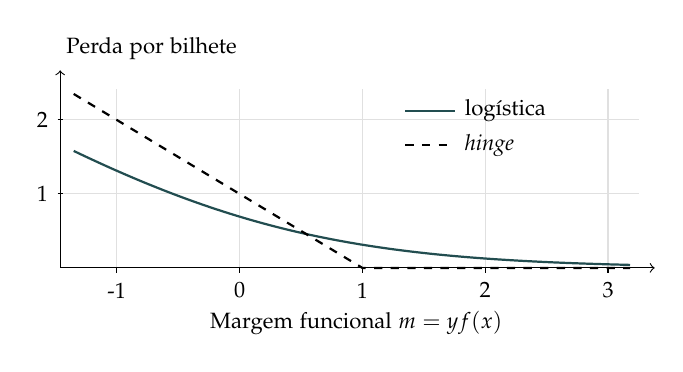
\begin{tikzpicture}[x=1.56cm,y=0.94cm,font=\footnotesize]
\foreach \x in {-1,0,1,2,3} {\draw[black!12] (\x,0)--(\x,2.42);\draw (\x,0)--(\x,-.07) node[below]{\x};}
\foreach \y in {1,2} {\draw[black!12] (-1.45,\y)--(3.25,\y);\draw (-1.48,\y)--(-1.44,\y) node[pos=0,left]{\y};}
\draw[->](-1.46,0)--(3.38,0);\draw[->](-1.46,0)--(-1.46,2.67);
\node[anchor=west] at (-1.49,2.97) {Perda por bilhete};
\node at (.95,-.74) {Margem funcional \(m=yf(x)\)};
\draw[tinta,thick,domain=-1.35:3.18,samples=100] plot (\x,{ln(1+exp(-\x))});
\draw[black,thick,dashed] (-1.35,2.35)--(1,0)--(3.18,0);
\draw[tinta,thick] (1.35,2.12)--(1.75,2.12) node[right,black]{logística};
\draw[black,thick,dashed] (1.35,1.66)--(1.75,1.66) node[right,black]{\emph{hinge}};
\end{tikzpicture}\par
{\footnotesize\raggedright Nas duas curvas, uma margem positiva corresponde à letra certa. Para a \emph{hinge}, a partir de \(m=1\) a cobrança por aquele exemplo chega a zero.\par}
\end{minipage}\par\addvspace{7pt}}

\newlanguage\brasil
\language=\brasil
\lefthyphenmin=2\righthyphenmin=3
\hyphenation{a-pren-da a-pren-de-mos a-pren-der a-pren-di-do a-pren-di-zes a-pren-di-za-do a-pren-di-za-gem pro-ba-bi-li-da-de pro-ba-bi-li-da-des dis-tri-bui-ção dis-tri-bui-ções ob-ser-va-ção ob-ser-va-ções ex-pe-ri-men-to ex-pe-ri-men-tos lan-ça-men-to lan-ça-men-tos hi-pó-te-se hi-pó-te-ses atu-a-li-za-ção atu-a-li-za-ções ge-ne-ra-ti-vo ge-ne-ra-ti-vos dis-cri-mi-na-ti-vo dis-cri-mi-na-ti-vos ve-ros-si-mi-lhan-ça e-xem-plos fre-quên-cia fre-quên-cias in-te-li-gên-cia in-te-li-gen-te in-de-pen-dên-cia in-de-pen-den-tes in-de-pen-den-te-men-te in-for-ma-ção in-for-ma-ções ne-ces-sá-rio ne-ces-sá-ria con-di-ci-o-nal con-di-ci-o-nais co-nhe-ci-men-to re-sul-ta-do re-sul-ta-dos ex-pe-ri-men-ta-dor es-ti-ma-ti-va es-ti-ma-ti-vas ge-ne-ra-li-zar co-e-fi-ci-en-te co-e-fi-ci-en-tes pre-vi-são pre-vi-sões con-ti-nu-ar con-ti-nua con-si-de-rar lo-ga-rit-mo lo-ga-rit-mos di-fe-ren-ça di-fe-ren-tes re-gres-são mul-ti-pli-ca-ção co-e-rên-cia pro-por-ci-o-nal neu-tra-li-da-de su-fi-ci-en-te su-fi-ci-en-tes pro-pri-e-da-de pro-pri-e-da-des exa-ta-men-te com-ple-ta-men-te con-ti-nua-rão per-gun-ta per-gun-tas clas-si-fi-ca-dor clas-si-fi-ca-do-res en-tro-pia in-cer-te-za dis-tri-bu-i-ção ex-pe-ri-men-ta-do-res re-pre-sen-tar de-ter-mi-nam con-di-ci-o-nan-do pa-râ-me-tros dis-po-ni-bi-li-da-de}

